%% ----------------------------------------------------------------
%% ObjectDetection.tex
%% ---------------------------------------------------------------- 
\chapter{Object Detection} \label{Chapter:ObjectDetection}

Object detection is the natural extension to the image classification problem. In image classification, for each sample there is a single output denoting the class of the sample. In mathematical notation for each sample $X$, the model $\phi$, $\phi(X)$, gives as output an $N-$vector $P_x=(p_1,p_2,...,p_N)$\footnote{$\sum^N_i p_i=1$}, where each element indicates the probability of the sample belonging in class $n_i \in N$. Object detection pushes this task a bit further by classifying and localising an instance in the image, instead of simply making a prediction. Therefore, for each sample query the output includes the predicted class and a set of coordinates that define a bounding box around the object; there could be more than one predictions for a single image. Despite that traditional object detection includes class prediction and a rectangle bounding box around the class, the vision community evolved object detection to image segmentation and instance segmentation. In image segmentation, the model is called to classify images pixel-wise where each pixel represents a class, while in instance segmentation the model segments the observed classes in objects and background. While object detection had started years prior deep learning's revolution, the most significant and robust algorithms have a deep learning approach. In general, deep learning based object detectors are divided in \textbf{\textit{double stage detectors}} and \textbf{\textit{single stage detectors}}. An overview of these methods will be given in the next sections along with the most significant models. 

\begin{figure}[!htb]
  \centering
  \subfigure[Classification.]{
    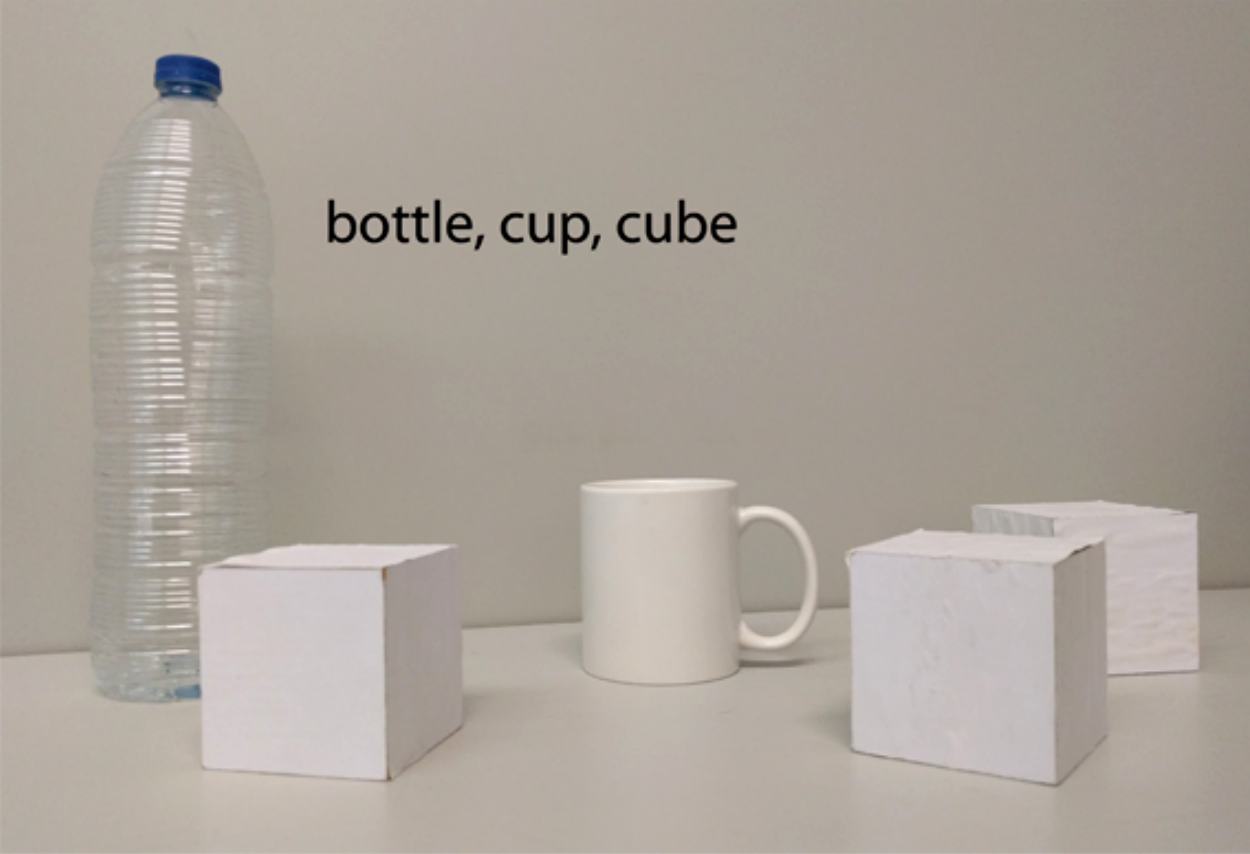
\includegraphics[width=4cm]{images/ch2/fig1_1.png}
    \label{fig1_1}
  }
  \subfigure[Detection (classification + localisation).]{
    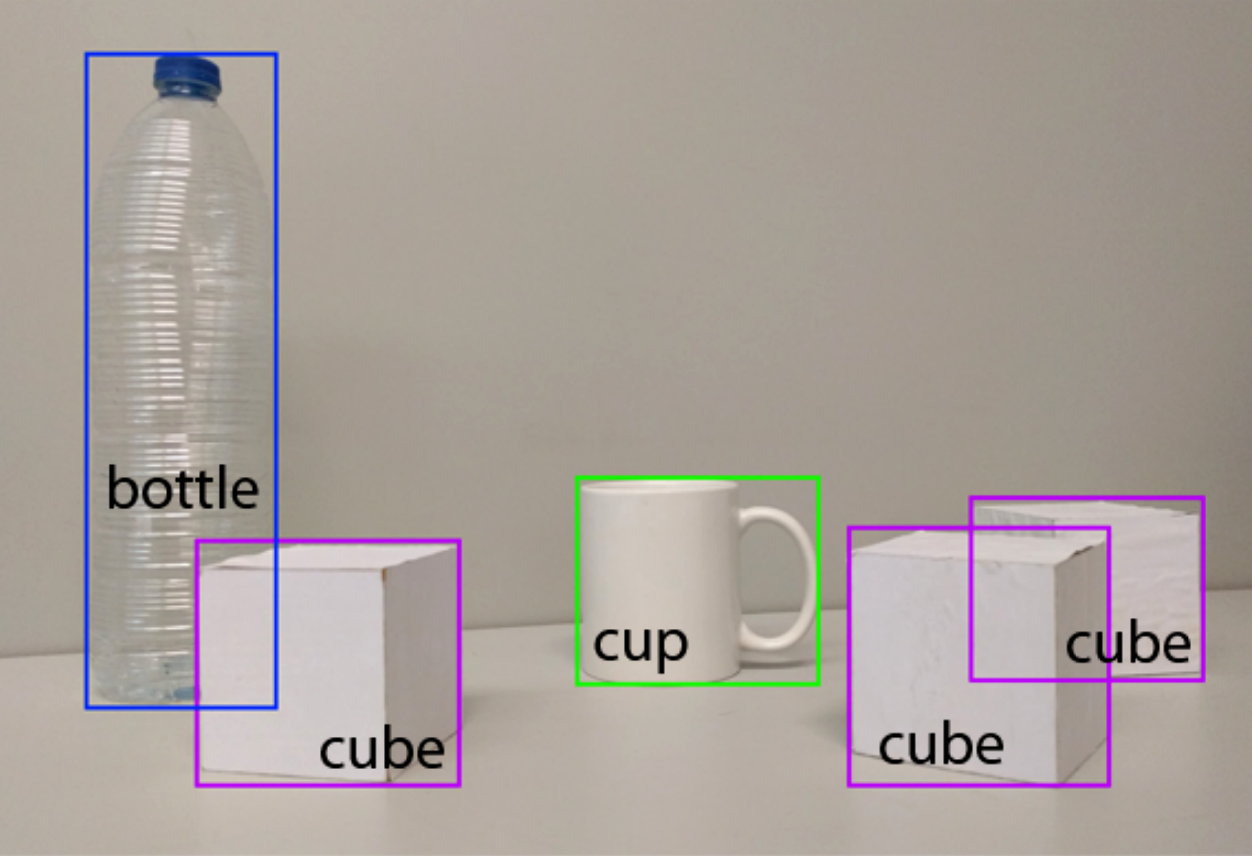
\includegraphics[width=4cm]{images/ch2/fig1_2.png}
    \label{fig1_2}
  }
  
    \subfigure[Image segmentation.]{
    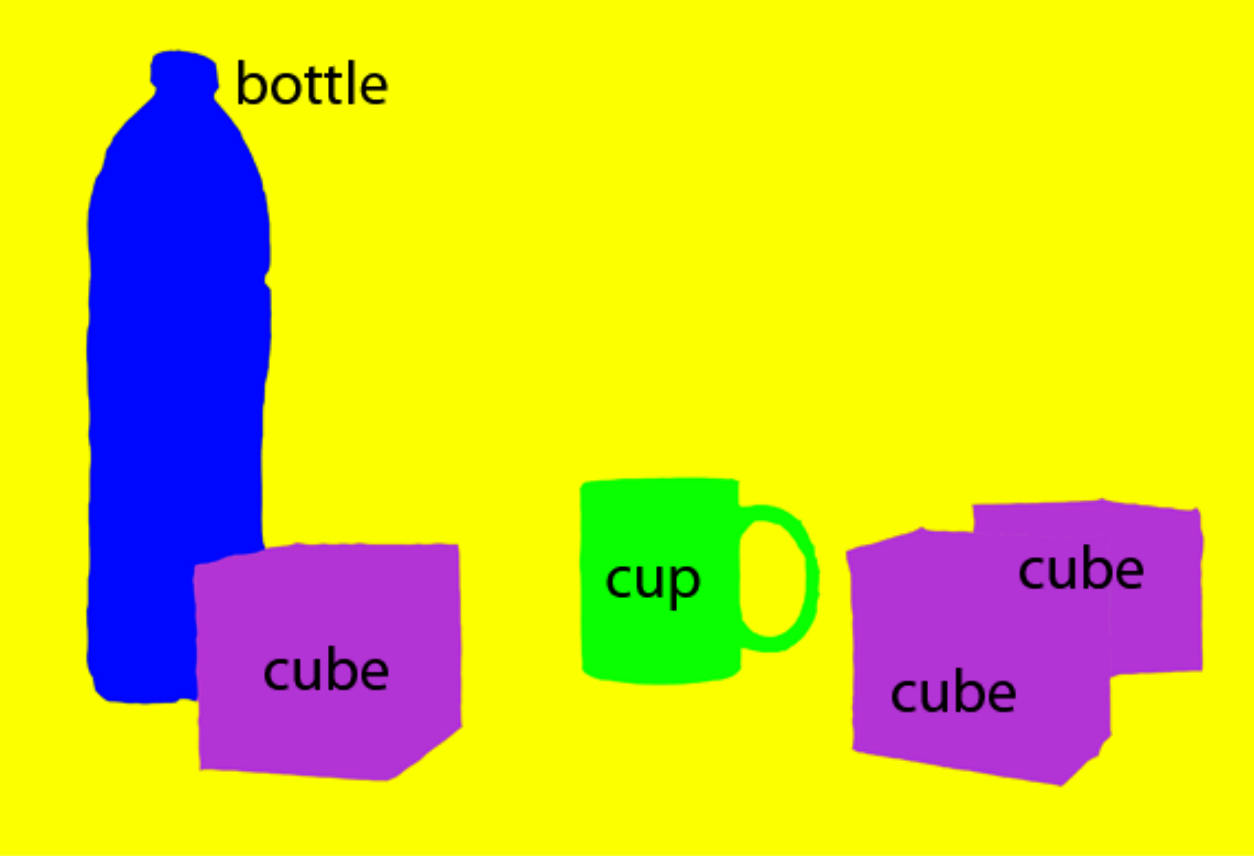
\includegraphics[width=4cm]{images/ch2/fig1_3.png}
    \label{fig1_3}
  }
    \subfigure[Instance segmentation.]{
    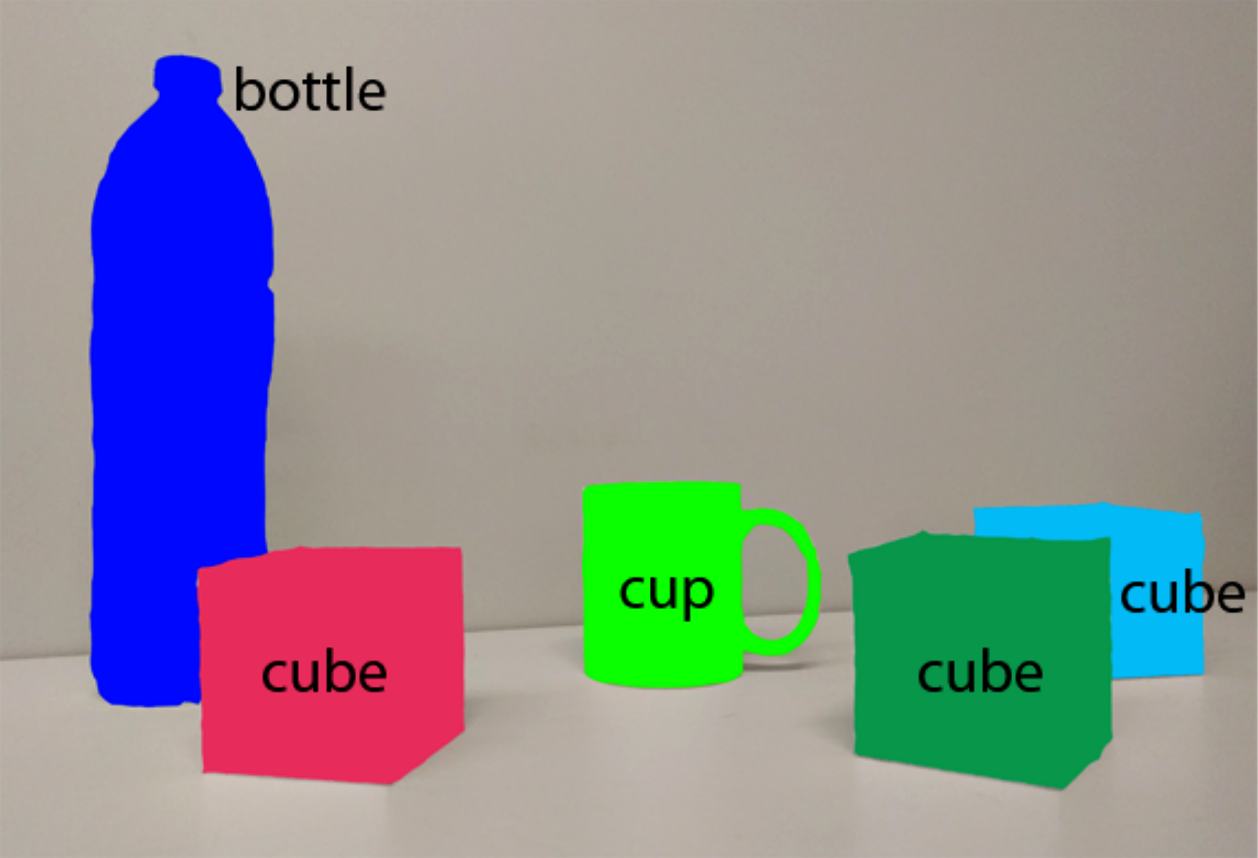
\includegraphics[width=4cm]{images/ch2/fig1_4.png}
    \label{fig1_4}
  }
  \caption{Each task provides semantically richer information (Reproduced from \cite{garcia1704review}).}
  \label{fig1}
\end{figure}

\section{Double-Stage Detectors}

The detection process in double stage or \textbf{\textit{region proposal based detectors}}, can be split in two parts. The first part generates class-agnostic regions of interest (RoIs) with a bounding box around them and the second part predicts the class of each proposed RoI and refines the bounding box around it. It's worth presenting a very popular method in double stage detectors called "R-CNN: Regions with CNN features" (\cite{girshick2014rich}) and its successors Fast R-CNN (\cite{girshick2015fast}) and Faster R-CNN (\cite{ren2015faster}) as Faster R-CNN still stays in fashion due to its high performance.

\subsection{R-CNN}
Before R-CNN was published, object detection was in stagnation without any significant improvement. R-CNN was the first method, that outperformed the previous state-of-the-art CNN method, OverFeat (\cite{sermanet2013overfeat}), increasing accuracy by a big margin. Specifically, R-CNN achieved a mean average precision (mAP) of 31.4\% on ILSVRC2013 (\cite{deng2009imagenet})dataset, over OverFeat which had the previous best result 24.3\%.

R-CNN consists of three parts. The first part generates 2000 class-agnostic regions of interest using selective search (\cite{uijlings2013selective}) with most of them being negative examples. Each proposed region of interest, acts as a potential detection defined by its bounding box. Then, these proposals are warped to a fixed size in order to match architecture's input size criteria. 
The second part is a CNN, pre-trained on the ImageNet dataset (fine-tuned on the new data), and acts as a feature extractor from its last fully connected layer.
The 4096-dimensional extracted features from each RoI, are then classified by class-specific SVMs (plus background) in the last step. After a detection is scored, class-specific box regressors regress the bounding box offsets resulting in a refined bounding box.

\begin{figure}[!htb]
  \centering
  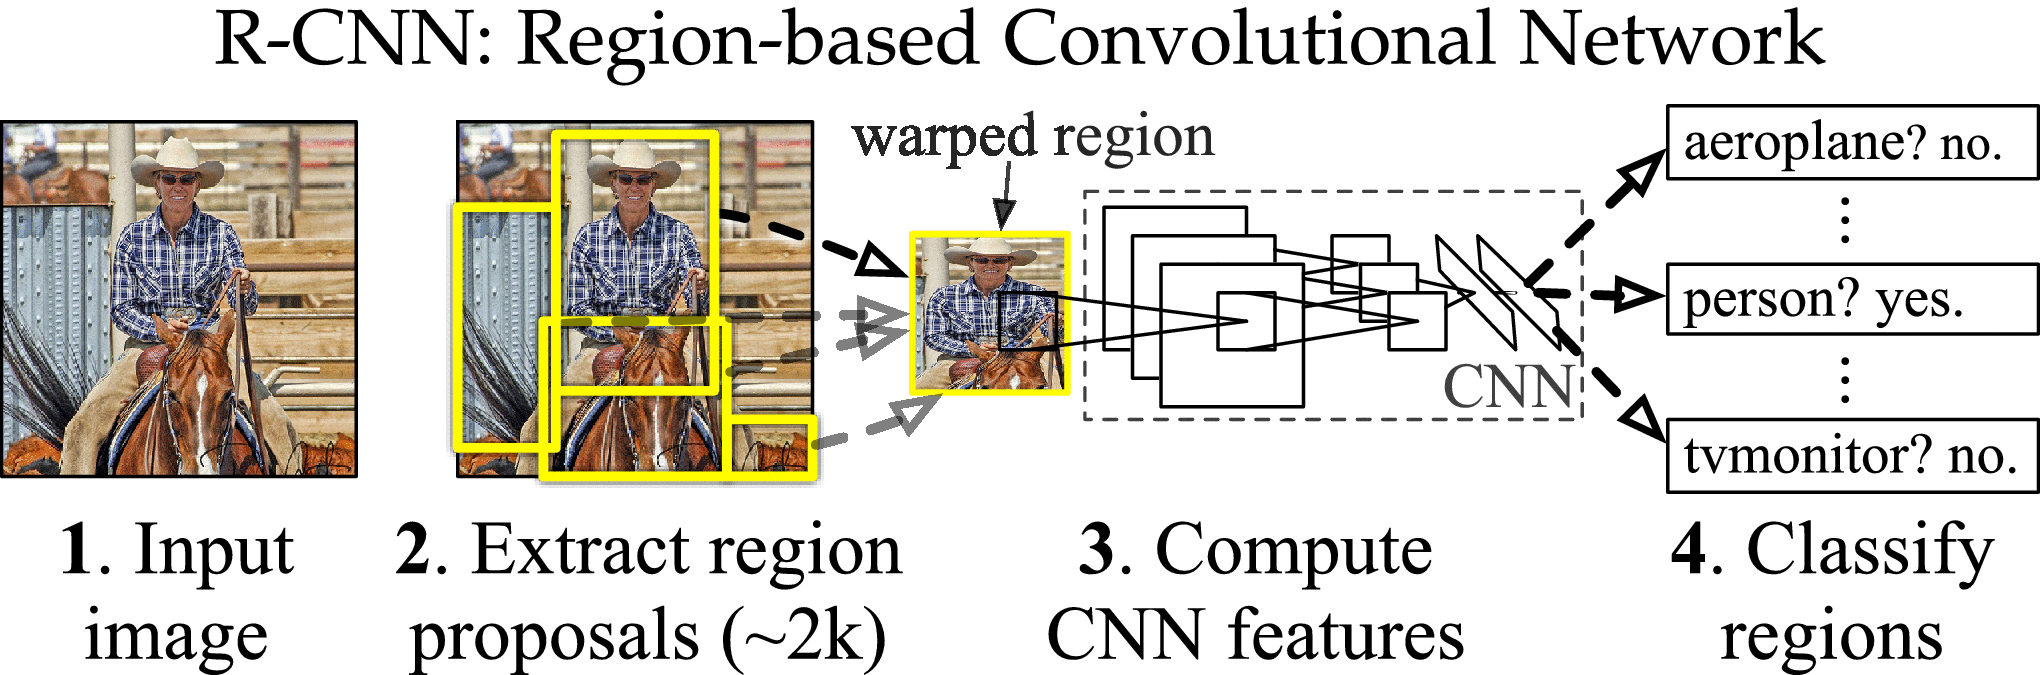
\includegraphics[width=12cm]{images/ch2/fig2.png}
  \caption{R-CNN pipeline as presented in \cite{girshick2014rich}.}
  \label{fig2}
\end{figure}

Although, R-CNN increased performance margin strikingly, has the following notable drawbacks:

\begin{itemize}
  \item The selective search is a heuristic based algorithm, thus it is unable to learn anything during the training procedure. 
  \item Training time takes a vast amount of time and space considering that for each image 2000 proposals have to be fed to the network. Since training it is a multi-stage pipeline, extracted features have to be cached on disk before passed to the SVMs and box regressors. Notice that since the majority of samples are negatives, the authors adopted hard negative mining forcing the model to focus on hard examples (\cite{felzenszwalb2009object}) in order to accelerate convergence.
  \item It is not suitable for real time applications as it has a GPU test rate of  47 seconds/images, when OverFeat was 9x times faster (\cite{girshick2015fast}). 
\end{itemize}

\subsection{Fast R-CNN}
Fast R-CNN was introduced as the improved version of R-CNN, where the multi-stage network was replaced by a single-stage pipeline able to be trained in one stage.

\begin{figure}[!htb]
  \centering
  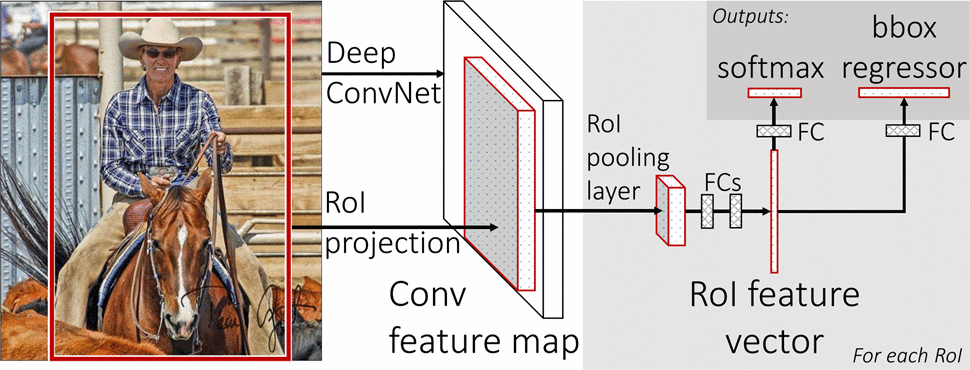
\includegraphics[width=12cm, height=3cm]{images/ch2/fig3.png}
  \caption{Fast R-CNN pipeline as presented in \cite{girshick2015fast}.}
  \label{fig3}
\end{figure}

To achieve this, Faster R-CNN adopted a method from SPPnet (\cite{he2015spatial}) called RoI pooling. R-CNN was handling proposals by warping them into a fixed size and feeding them into the network one by one. On the contrary, SPPnet and Faster R-CNN compute varying size feature maps of the entire image instead of warped region proposals. Each feature map contains RoI information in a four-tuple $(r,c,h,wR-CNN)$, where $r, c:$ top-left corner and $w, h:$ width and height. Fixed size RoI feature vectors are pooled from variable size feature maps through RoI pooling. \fref{fig4} presents how RoI pooling extracts fixed length feature vectors from feature maps with variable sizes. Moreover, the SVMs and the box regressors are replaced by a joint sibling layer. One layer produces the softmax probability over K + 1 background classes, while the other predicts offsets for the refined bounding boxes. \fref{fig3} illustrates an overview of the model. 

\begin{figure}[!htb]
  \centering
  \subfigure[Feature map with 2 RoIs.]{
    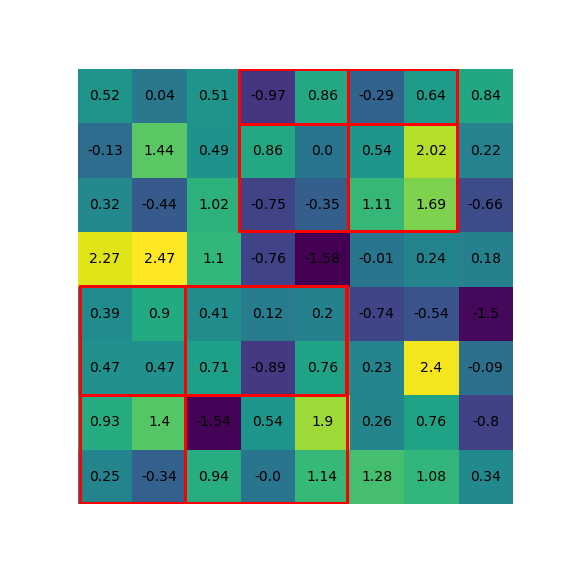
\includegraphics[width=6cm]{images/ch2/fig4_1.png}
    \label{fig1_1}
  }
  \subfigure[RoIs after RoI pooling.]{
    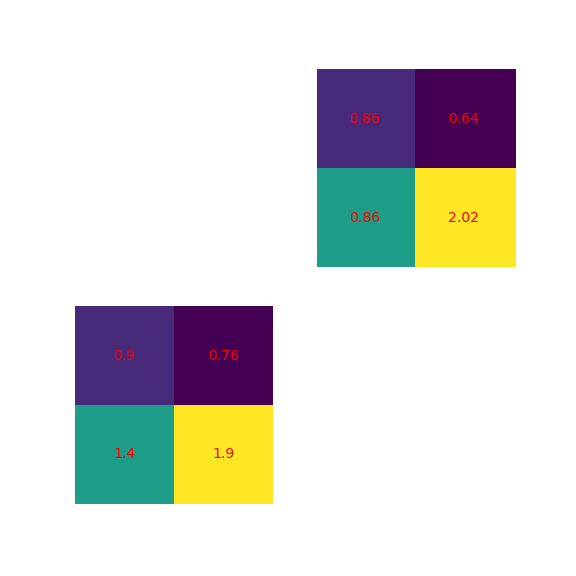
\includegraphics[width=6cm]{images/ch2/fig4_2.png}
    \label{fig1_2}
  }
  \caption{In order to extract vectors of fixed length, different sized proposed RoIs are divided in a fixed number of bins appropriately.}
  \label{fig4}
\end{figure}

By feeding the entire image into the network instead of $\sim$2k proposals one by one, the network avoids redundant computations since a lot of proposals are overlapping each other, hence it is more efficient than its predecessor both in terms of time and memory. Specifically, it is 10x faster than R-CNN in training time and 213x in testing. Furthermore, a joint loss $\mathcal{L}=\mathcal{L}_{cls}+\mathcal{L}_{reg}$ from the softmax and the regression layers optimises the network.

\subsection{Faster R-CNN}
After the replacement of the SVMs with softmax functions, Fast R-CNN was the state-of-the-art object detector, based almost entirely on convolutional neural networks. Its major disadvantage was that the region proposal method, selective search, was not a learning method but a heuristic approach. Soon, this was fixed by the introduction of Faster R-CNN (\cite{ren2015faster}) which entirely dismissed selective search and replaced it with a trainable region proposal network (RPN). RPN, is a CNN where the network's output is attached to a class predictor and a box regressor. The class predictor has only two classes (object, not object), thus the networks is trained to propose regions of interest by their "\textit{objectness}". The rest of the network is adopted by the Fast R-CNN pipeline. Faster R-CNN is classified in the double-stage detectors even if the region proposal method is not decoupled, anymore, from the main pipeline, due to it's 4-step alternate training:
 
\begin{enumerate}
  \item RPN is initialised with the ImageNet weights and fine-tuned for the region proposal task.
  \item The detector (Fast R-CNN) is initialised with the ImageNet weights and fine-tuned for the detection task, with the proposed regions of interest from the RPN (the two models do not share any convolutional layers).
  \item The detector is used to initialise the RPN training, with keeping constant weights coming from shared layers and updating only weights from unique layers. At this point the two models share convolutional layers.
  \item Keeping constant weights from common convolutional layers, detector's unique layers are fine-tuned. 
\end{enumerate}

Faster R-CNN's greatest success is that it consists of a single-stage end-to-end trainable network, entirely based on CNNs with an inference time of 5 FPS.


\section{Single-Stage Detectors}
The downside of double-stage detectors is that training time is split in two separate parts, the region proposal and the detection part, hindering real-time detection. Single-stage detectors or \textbf{\textit{regression/classification based detectors}} have the advantage of being really fast. The main reason is that instead of making class predictions and refining bounding boxes on already proposed regions, apply global rules in every pixel inferring relevant detections without intermediate mechanisms. In this category, the most important algorithms are the SSD (\cite{liu2016ssd}), the YOLO model (\cite{redmon2016you}) and RetinaNet (\cite{lin2017focal}) and will synopsised in the next pages.
 
 \subsection{YOLO}
 YOLO, developed by \cite{redmon2016you} (followed by the improved versions of YOLOv2 \cite{redmon2017yolo9000} and YOLOv3 \cite{redmon2018yolov3}) is a model known for its rapid inference 
 rates ranging between 20-220FPS (depending the backbone implementation) based entirely on Darknet; a network developed by Redmon.
 
 The idea behind YOLO is to obtain detections from each pixel instead of relying on region proposal methods. An image $W\times H$ is fed into the backbone network and the output is an activation feature map of size $S\times S$. Each pixel in the given feature map, represents an area in the original image of $\frac{W}{S} \times \frac{H}{S}$. Also, each cell on the grid is responsible for detecting an object that has its center on that cell. For example, if an object lies in the bottom right corner of the original image, pixel $(S,0)$ on the feature map, is responsible for its detection. If an object lies in the middle of the image, pixel $(\frac{S}{2},\frac{S}{2})$ is responsible for its detection. 
 
\begin{figure}[!htb]
  \centering
  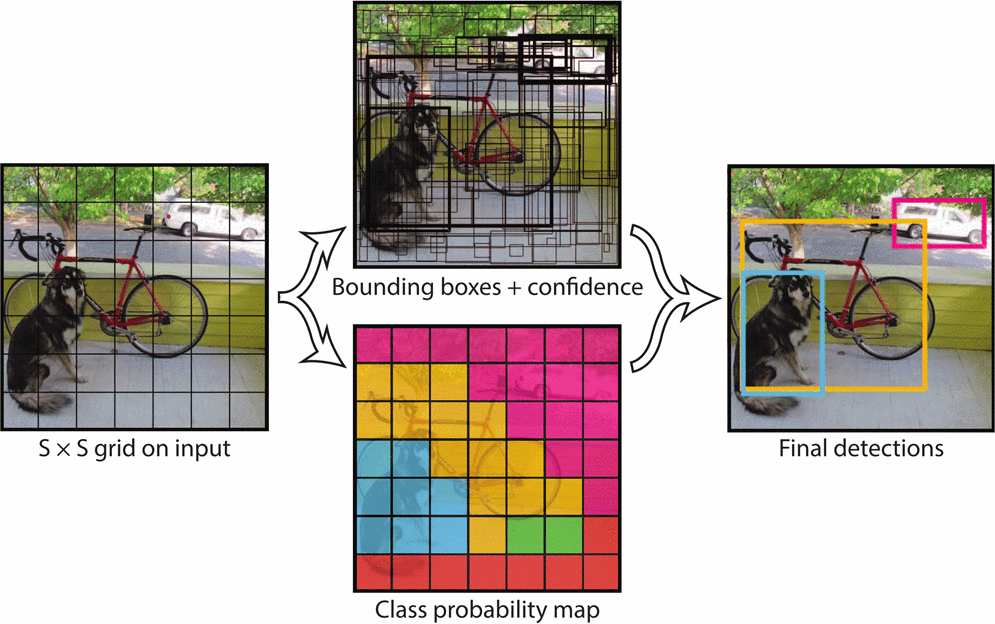
\includegraphics[width=12cm]{images/ch2/fig5.png}
  \caption{A schematic representation of how grid cells detect objects. Reproduced from \cite{redmon2016you}.}
  \label{fig5}
\end{figure} 
 
The actual size of the feature map sized $S\times S$ is a five-tuple $S\times S \times B\times(5+C)$ tensor, where 5 in parentheses implies four coordinates and an objectness score, C is an one-hot encoded vector which indicates the class and B is the number of different detections. As a matter of fact, each cell makes B predictions of arbitrary size and the final detection is the one with the biggest $p_obj$ confidence score. The last layer produces a conditional probability $p(c_i|obj)$ and the refined bounding box.

The next versions of YOLO, could make predictions in intermediate layers (from feature maps of different size) enabling detection in various scales. 
 
\subsection{SSD}
Single Shot Detector (or SSD) was published right after YOLO, by \cite{liu2016ssd} and aimed to solve YOLO problems. SSD follows an architecture based on VGG16 (as Faster R-CNN) and operates as YOLO. The first version of Redmon's detector had difficulties detecting objects in different scales due to multiple pooling layers, thus SSD was aiming to fix this. 

Regarding its architecture, an additional network is attached right after the fifth convolutional block of the VGG16. Classification and regression happens on several feature maps of different size from finer to coarser resolutions. Moreover, grid cells, instead of predicting the conditional class probability $p(c_i|obj)$, predict $p(c_i)$, thus it is necessary the introduction of one more class that acts as background. While SSD could achieved higher mAP than YOLO with similar detection rates and could detect objects in multiple scales, it was facing difficulties in small object detection but this could be relieved by altering the backbone network.  \fref{fig6} shows an overview of the model.
 
\begin{figure}[!htb]
  \centering
  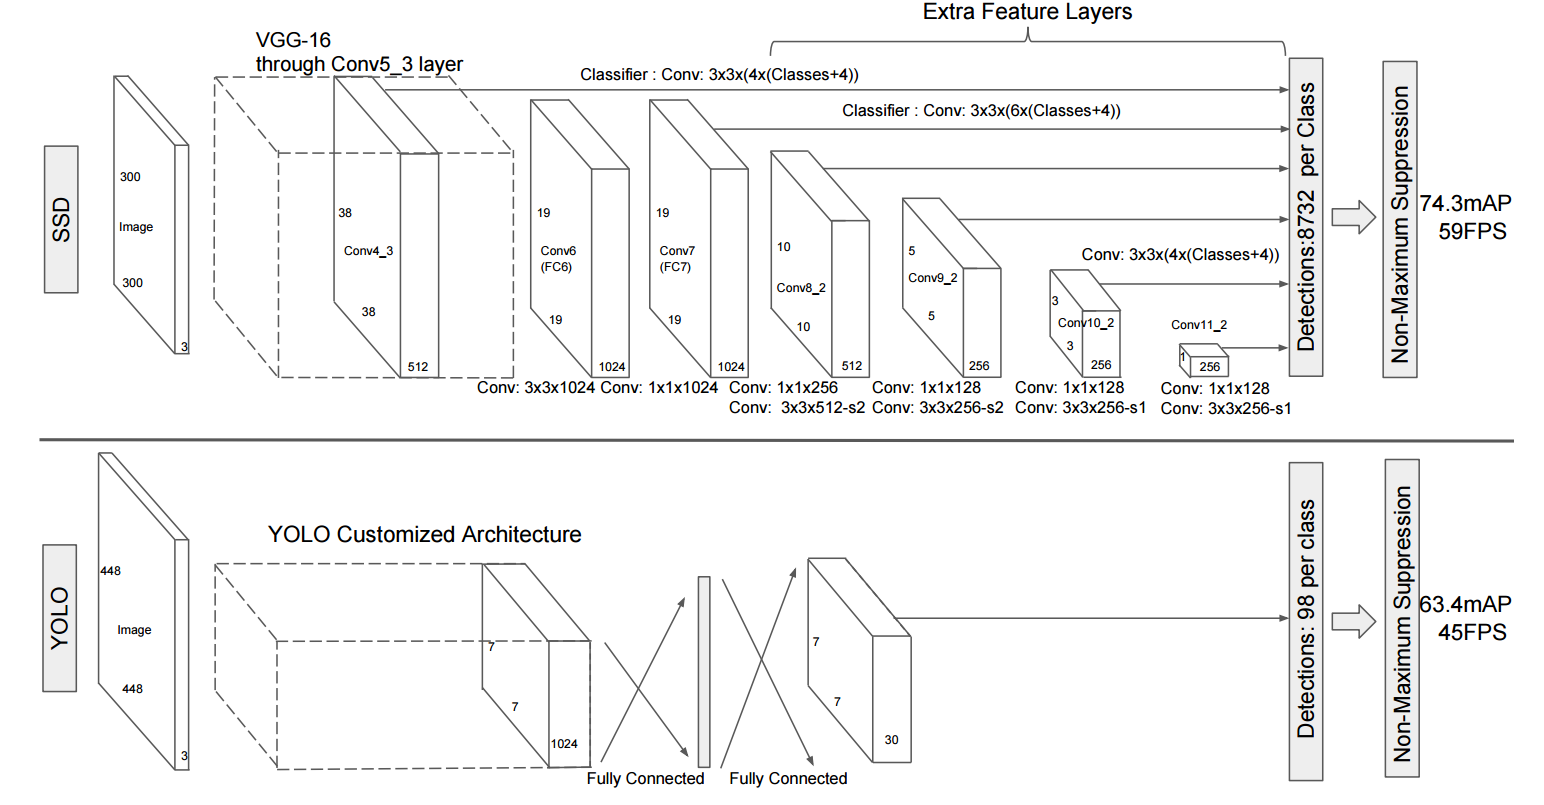
\includegraphics[width=12cm]{images/ch2/fig6.png}
  \caption{A comparison between SSD and YOLO architectures. Reproduced from \cite{liu2016ssd}.}
  \label{fig6}
\end{figure} 
 
The previous sections in this chapter, summarised an overview of the most widely used object detectors, the novelties in their architectures, their advantages along with their shortcomings. One the one hand, double-stage detectors produce region proposals and deal with detection in latter stage, and on the other, single-stage detectors divide the images in a grid and produce a bounding box (or not) around a grid cell depending on a probability $p(obj)$. The trade-off between these object detector families is that double-stage detectors usually achieve higher accuracies, while single-stage detectors are much faster. The following sections provide information about technical specifications and concepts met in every object detector in a more detailed manner.

\section{Prior Bounding Boxes (Anchors)}
Anchors act as reference boxes of predefined size around RoIs; the box regressors on the final layer, try to refine them for an accurate localisation. Instead of producing new coordinates for every detection, predicting the offsets $(\Delta x, \Delta y, \Delta w, \Delta h)$ of the predefined bounding box is much more efficient. These anchor boxes can be more than one with different scales and ratios; in other words, it is easier refining an elongated vertical box around a person rather than a square box. 

Usually, most models define by default 9 anchor boxes with scales of $(2^0, 2^{1/3}, 2^{2/3})$ and ratios of $(1\!:\!2,1\!:\!1,2\!:\!1)$, but this depends on the variation of objects in the dataset. A common practice to find the most representatives scales and ratios is to apply K-means clustering over the dataset.

In single-stage detection, the spatial size of the feature map where the classifier and box predictor are attached to, depends on the depth of the particular convolutional layer. \fref{fig7} shows an $8\times8$ feature map where each grid cell tries to fit best 9 anchor boxes of area $K\times K$. Each grid cell represents a spatial area of $(\frac{W}{8}, \frac{H}{8})$ in the original image. Grid cell $(3,3)$ will make a positive detection if $p(obj)$ is bigger than a certain threshold; if $p(obj)$ on $(4,3)$ exceeds that threshold as well, new prediction's center has 8 pixel distance from the previous. Therefore, this feature map's predictions are characterised by a stride = 8. More dense predictions can be achieved by feature maps of bigger spatial size. Hence pooling layers have a direct effect on prediction density.

 \begin{figure}[!htb]
  \centering
  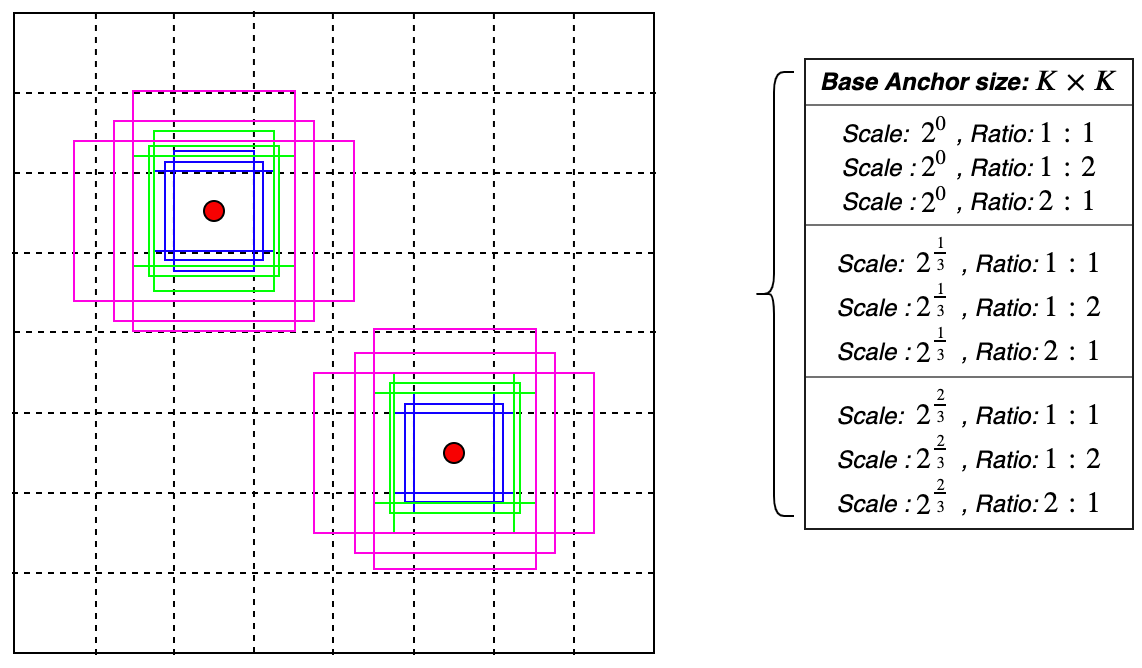
\includegraphics[width=7cm]{images/ch2/fig7.png}
  \caption{A typical topology with 9 anchors acting as prior bounding boxes.}
  \label{fig7}
\end{figure} 

In order to associate ground truth boxes with suitable anchors, each anchor gets assigned with the overlap between the anchor and the ground truth box that covers the most (if any). If the IoU overlap is more than 0.5, then this anchor should detect the object and it's called \textbf{\textit{positive anchor}}. If the IoU overlap is less than 0.4, that anchor should not make a a prediction and it's classified as a \textbf{\textit{negative anchor}}. During training, if an anchor is neither positive nor negative, it does not contribute to the overall loss. In inference mode, only the anchor with the biggest overlap will be proposed.

\section{Intersection Over Union}
Intersection over Union or Jaccard index, is an evaluation metric used to measure how accurately a predicted box match or overlaps the ground truth. As name indicates, the ratio between the intersection and the union of two boxes. In most tasks, as in PASCAL VOC challenge \cite{everingham2010pascal}, if the IoU between the detection and the ground truth is more than 0.5, the detection counts as a true positive.

\begin{figure}[!htb]
  \centering
  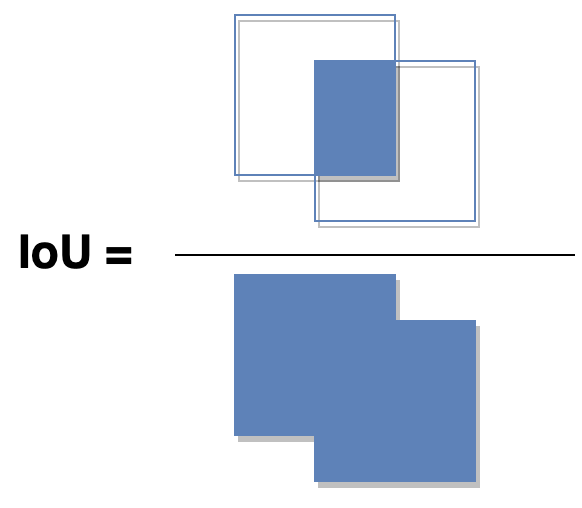
\includegraphics[width=3cm]{images/ch2/fig8.png}
  \caption{The Intersection over Union ratio.}
  \label{fig8}
\end{figure} 

\section{Non-Maximum Suppression}
Usually, objects extend much more in space rather than occupying only a grid cell on the feature map. Thus, many adjacent grid cells, by processing similar context information, may be triggered and produce multiple predictions referring to the same object. A post processing technique called non-maximum suppression (NMS) deals with this problem by suppressing the detections with IoU over a certain threshold. NMS algorithm can be summarised in the following steps:

\begin{itemize}
  \item In each cell, if $p(obj)>obj_{th}$ the anchor with the biggest IoU with the ground truth box will be proposed as prediction. 
  \item If there are overlapping predictions, with IoU greater than $NMS_{th}$, the detection with the highest $p(c_i|obj)$ will be proposed as the prediction, while the remaining predictions with be suppressed. 
\end{itemize}

That way NMS suppresses multiple predictions that most likely refer to the same object, but if there are objects that are really close to each other, and their detections have possibly an overlap greater than $NMS_{th}$, most of them will be falsely suppressed but one. 

\section{Multi-task Loss} 
\cite{ren2015faster}, in Faster R-CNN, introduced a coupled loss which combined both the loss from the classification and the regression task. During training, only positive and negative anchors contribute to the loss function; positive anchors in both classification and regression task while negatives only in classification.
The multi-task loss is a weighted combination of the smooth L1 loss and cross entropy.

\begin{equation}
  L(p_i,t_i) = \frac{1}{N_{cls}}\sum_i{L_{cls}(p_i,p_i^*)}+ \frac{\lambda}{N_{reg}}\sum_i p_i^*{L_{reg}(t_i,t_i^*)}
\end{equation} 

$N_{cls}$, and $N_{reg}$ are normalisation parameters, usually the number of instances in the SGD sample and $\lambda$ a balancing parameter. $p_i^*, p_i$ indicates the ground truth and predicted probability respectively, while $t_i^*, t_i$ is a four-tuple referring to the 4 ground truth and predicted coordinates that describe the bounding box.

\begin{equation}
    L_{cls}(p,p^*)= \bigg\{
    \begin{array}{ll}
      -log(p) & \text{if } p^*=1 \\
      -log(1-p) &  \text{otherwise}\\
    \end{array}
\end{equation}

Smooth L1 loss is claimed to be more robust to outliers (\cite{ren2015faster}) rather than L2 in which inappropriate learning rates result in exploding gradients. For similar values, or when the manhattan distance between $t_i, t_i^*$ is very small, smooth L1 is much smaller than L1. Additionally, for L1 greater than 1, it can be seen that gradients are constrained to 1. SSD uses the default formula for smooth L1 loss while Faster R-CNN adopts a parameter $\sigma$ which control the point between quadratic and linear loss. Large values of $\sigma$ convert smooth L1 loss to L2 loss.

\begin{equation}
    L_{reg}(t,t^*)= \bigg\{
    \begin{array}{ll}
      0.5\sigma^2(t-t^*)^2 & \text{if } |t-t^*|\leq \frac{1}{\sigma^2} \\
      |t-t^*|-\frac{0.5}{\sigma^2} &  \text{otherwise} \\
    \end{array}
\end{equation}

The following equations show the adopted parameterisation for $t_i$, where $(x^*,y^*,w^*,h^*)$, $(x_a,y_a,w_a,w_h)$ and $(x,y,w,h)$ refer to ground truth, anchor and predicted boxes respectively. 

\begin{align}
t_x		&= (x-x_a)/w_a			&		t_y	&= (y-y_a)/h_a \\
t_w		&= log(w/w_a)			&		t_h 	&= log(h/h_a) \\
t_x^*		&= (x^*-x_a)/w_a		&		t_y^*	&= (y^*-y_a)/h_a \\
t_w^*	&= log(w^*/w_a)		&		t_h^*	&= log(h^*/h_a) 
\end{align}

\section{Focal Loss}
The number of bounding box priors covering the image, is usually very large, orders of magnitude greater than the number of instances in the image. This creates a class imbalance between negative and positive anchors. To address this class imbalance, \cite{lin2017focal}, introduced a weighted cross entropy loss named "focal loss". Prior to focal loss, the most widely adopted method to deal with class imbalance was Online Hard Example Mining explicitly showing the model the hard examples to calculate gradients according to them. Another strategy is feeding the model with a sampling ratio of 1:3 in positives and negatives samples.

Focal loss, down-weights cross entropy asymmetrically forcing the model to focus on hard examples, that is examples with low confidence $p$. $\gamma$ is the scaling factor, and $\alpha_t$ a balancing factor, the authors state that its precise form is not crucial.

\begin{equation}
    FL(p,p^*)= \bigg\{
    \begin{array}{ll}
      -a_t(1-p)^\gamma log(p) & \text{if } p^*=1 \\
      -a_tp^\gamma log(1-p) &  \text{otherwise}\\
    \end{array}
\end{equation}

\section{RetinaNet}
RetinaNet, was introduced as a single-stage adaptation of the Feature Pyramids Networks (FPN, \cite{lin2017feature}) with the enhancement of focal loss. It is the bridge between double-stage and single-stage detection, as it surpassed the performance of Faster R-CNN with detection rates similar to YOLO and SSD.

Detecting objects in different scales is a demanding task and the standard approach is using image pyramids as a solution. SSD made one of the first attempts in multi-scale object detection by exploiting network's pyramidal feature hierarchy. A convolutional network has the advantage of producing, in each layer, feature maps that get semantically richer with the depth of the layer. Pooling operations, result in feature maps, large in resolution but weak in information and more coarse feature maps but semantically rich, obtained from the deeper layers. RetinaNet exploits feature maps from intermediate network layers by combining large resolution semantically weak features with coarser, semantically stronger feature maps. \fref{fig9}, shows different types of pyramidal feature exploitation.

\begin{figure}[!htb]
  \centering
  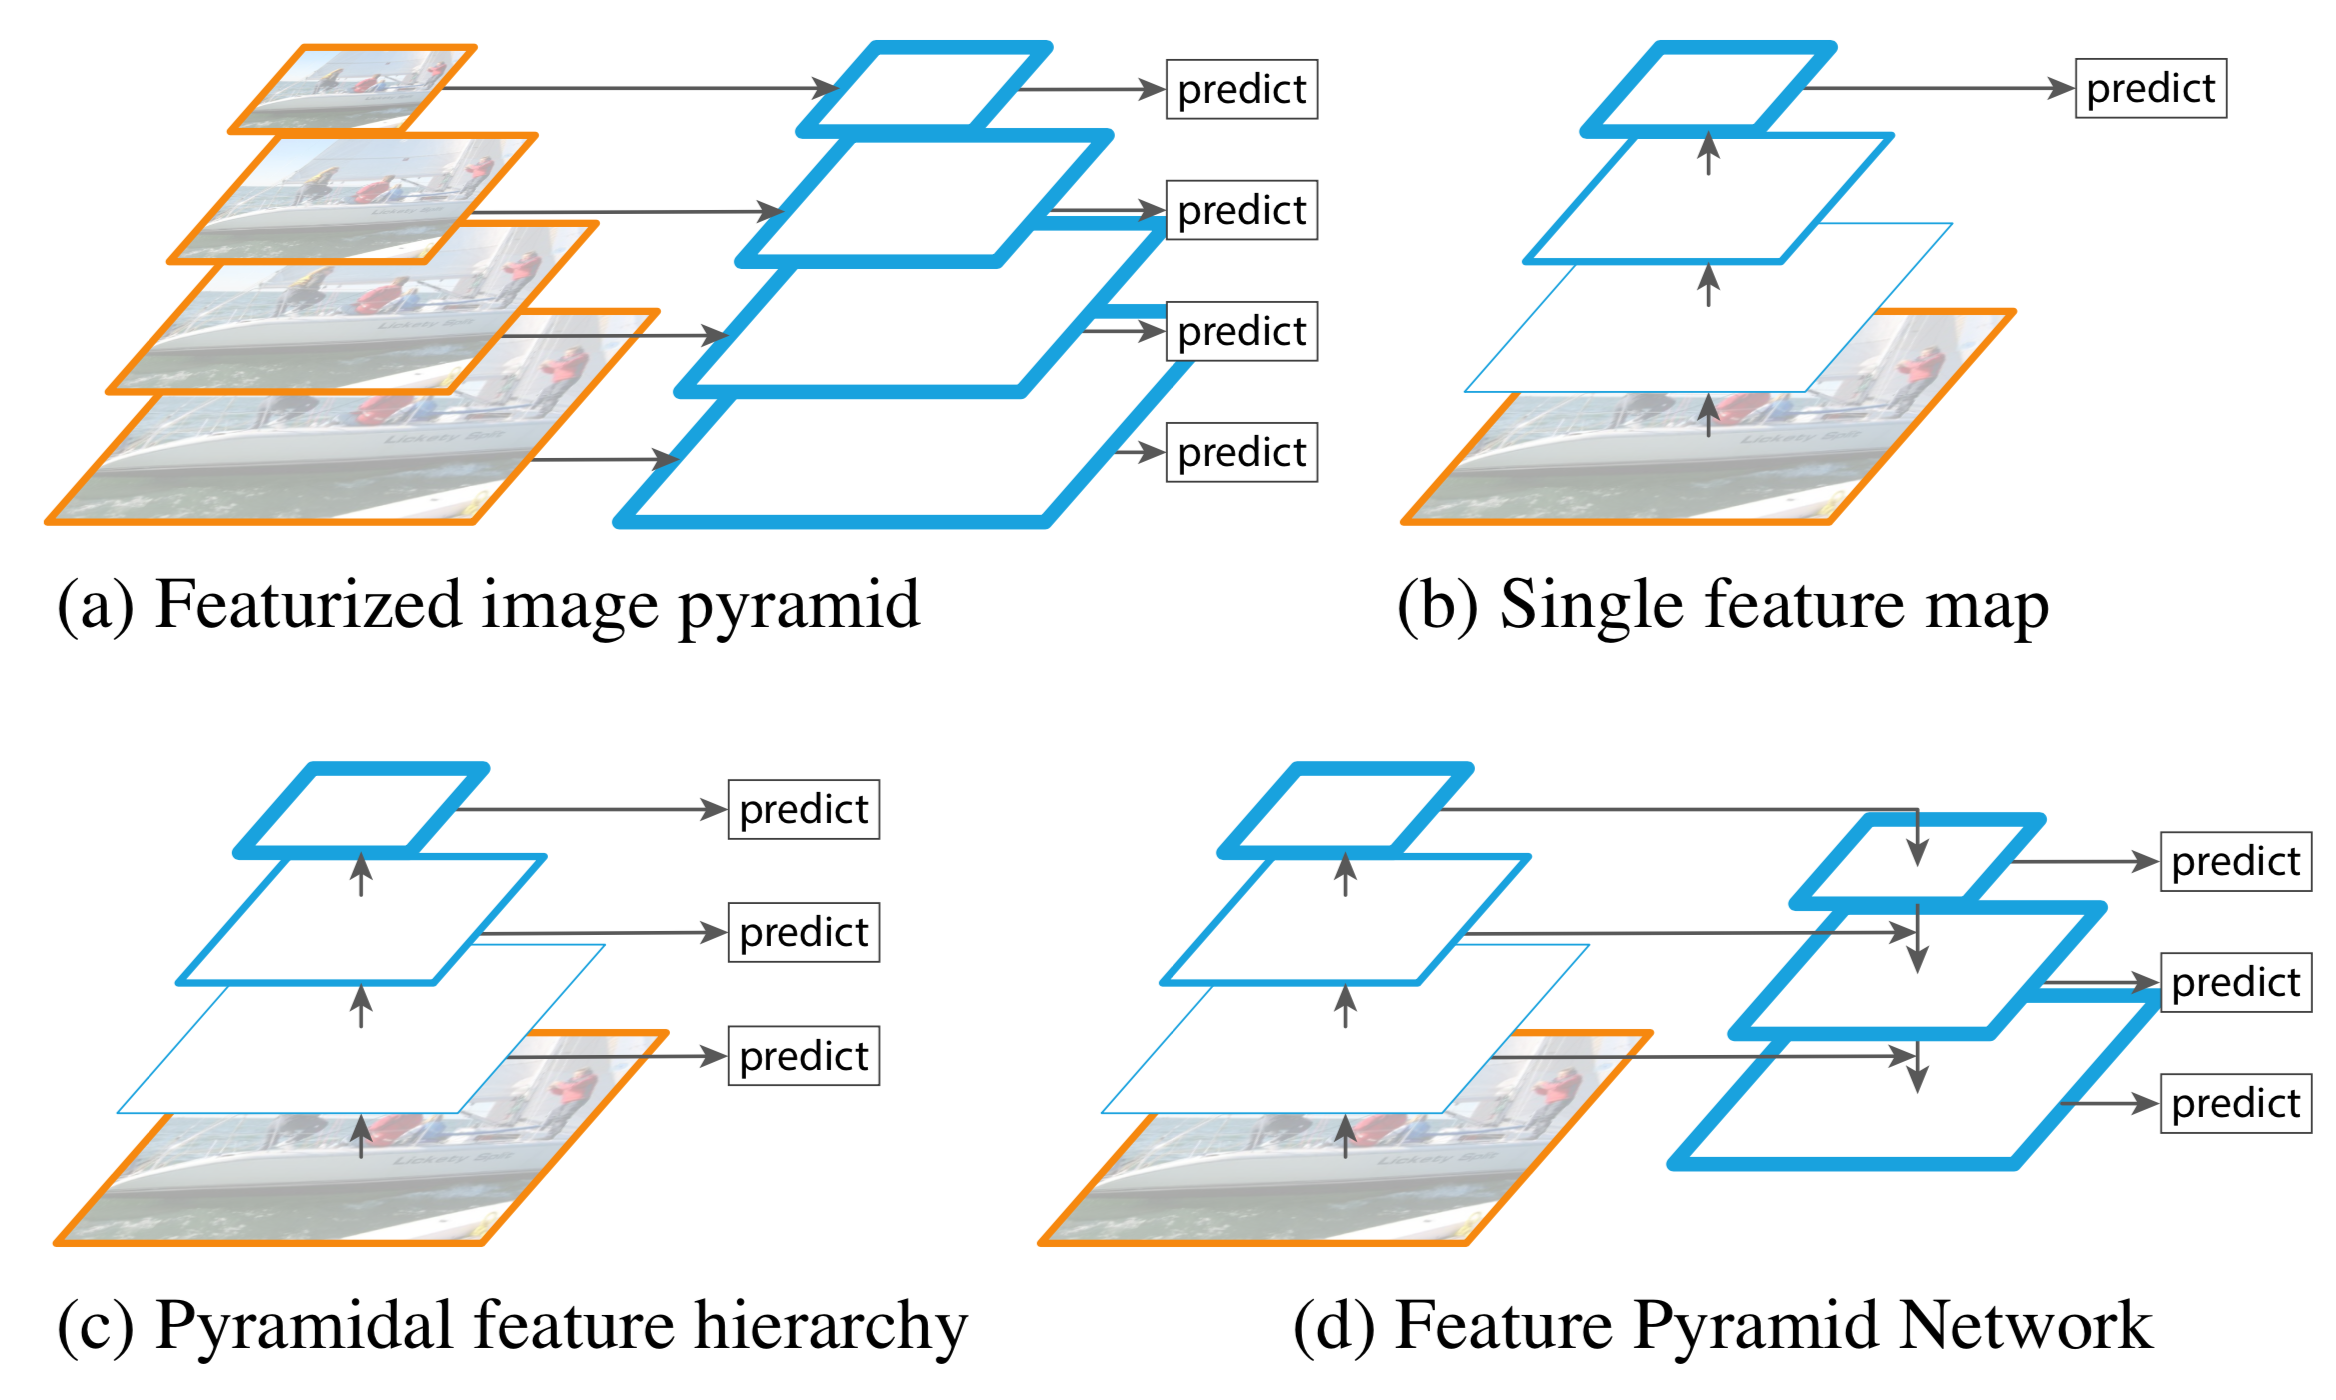
\includegraphics[width=12cm]{images/ch2/fig9.png}
  \caption{(a) Building an image pyramid by feeding an image in multiple scales, this is used to be a common practice but it is computationally infeasible. (b) Feeding an image and making predictions from the coarsest, very rich in information, feature map. It is a very fast method for making single scale predictions. (c) Detection in different scales by exploiting feature maps in the intermediate layers; it was adopted by the SSD. (d) The FPN method. Detects objects in different scales as a common SSD detector, but bottom layers are enriched with upsampled coarser, semantically stronger, top layers. Reproduced from \cite{lin2017feature}}
  \label{fig9}
\end{figure} 

\subsection{Architecture}
\fref{fig10} shows how the spatially larger feature maps are enriched by adding upsampled coarser maps. During the bottom-up pathway, the backbone network computes feature maps at several scales with the help of pooling operations. In the case of the VGG architecture, the model consists of 5 convolutional blocks and in the end of each convolutional block, the feature map is downscaled by 2 (the depth of the feature map depends on the architecture) resulting in the hierarchical features $(C_1, C_2, C_3, C_4, C_5)$. For the top-bottom pathway, the feature maps $C_i$ are obtained via lateral connections and convolved with $1\times1$ kernels to produce $C_{i_{reduced}}$ features of the same spatial size but with fixed depth. The coarser feature map is upsampled by the nearest neighbour method, and is added element-wisely with the $C_{i_{reduced}}$ maps. Each merged map, finally undergoes a $3\times3$ convolution to reduce the aliasing effect from upsampling. The result is a set of features downscaled by 2, $(P_1,P_2,P_3,P_4,P_5)$, where each $P_i$ contains information from deeper level features. 

\begin{figure}[!htb]
  \centering
  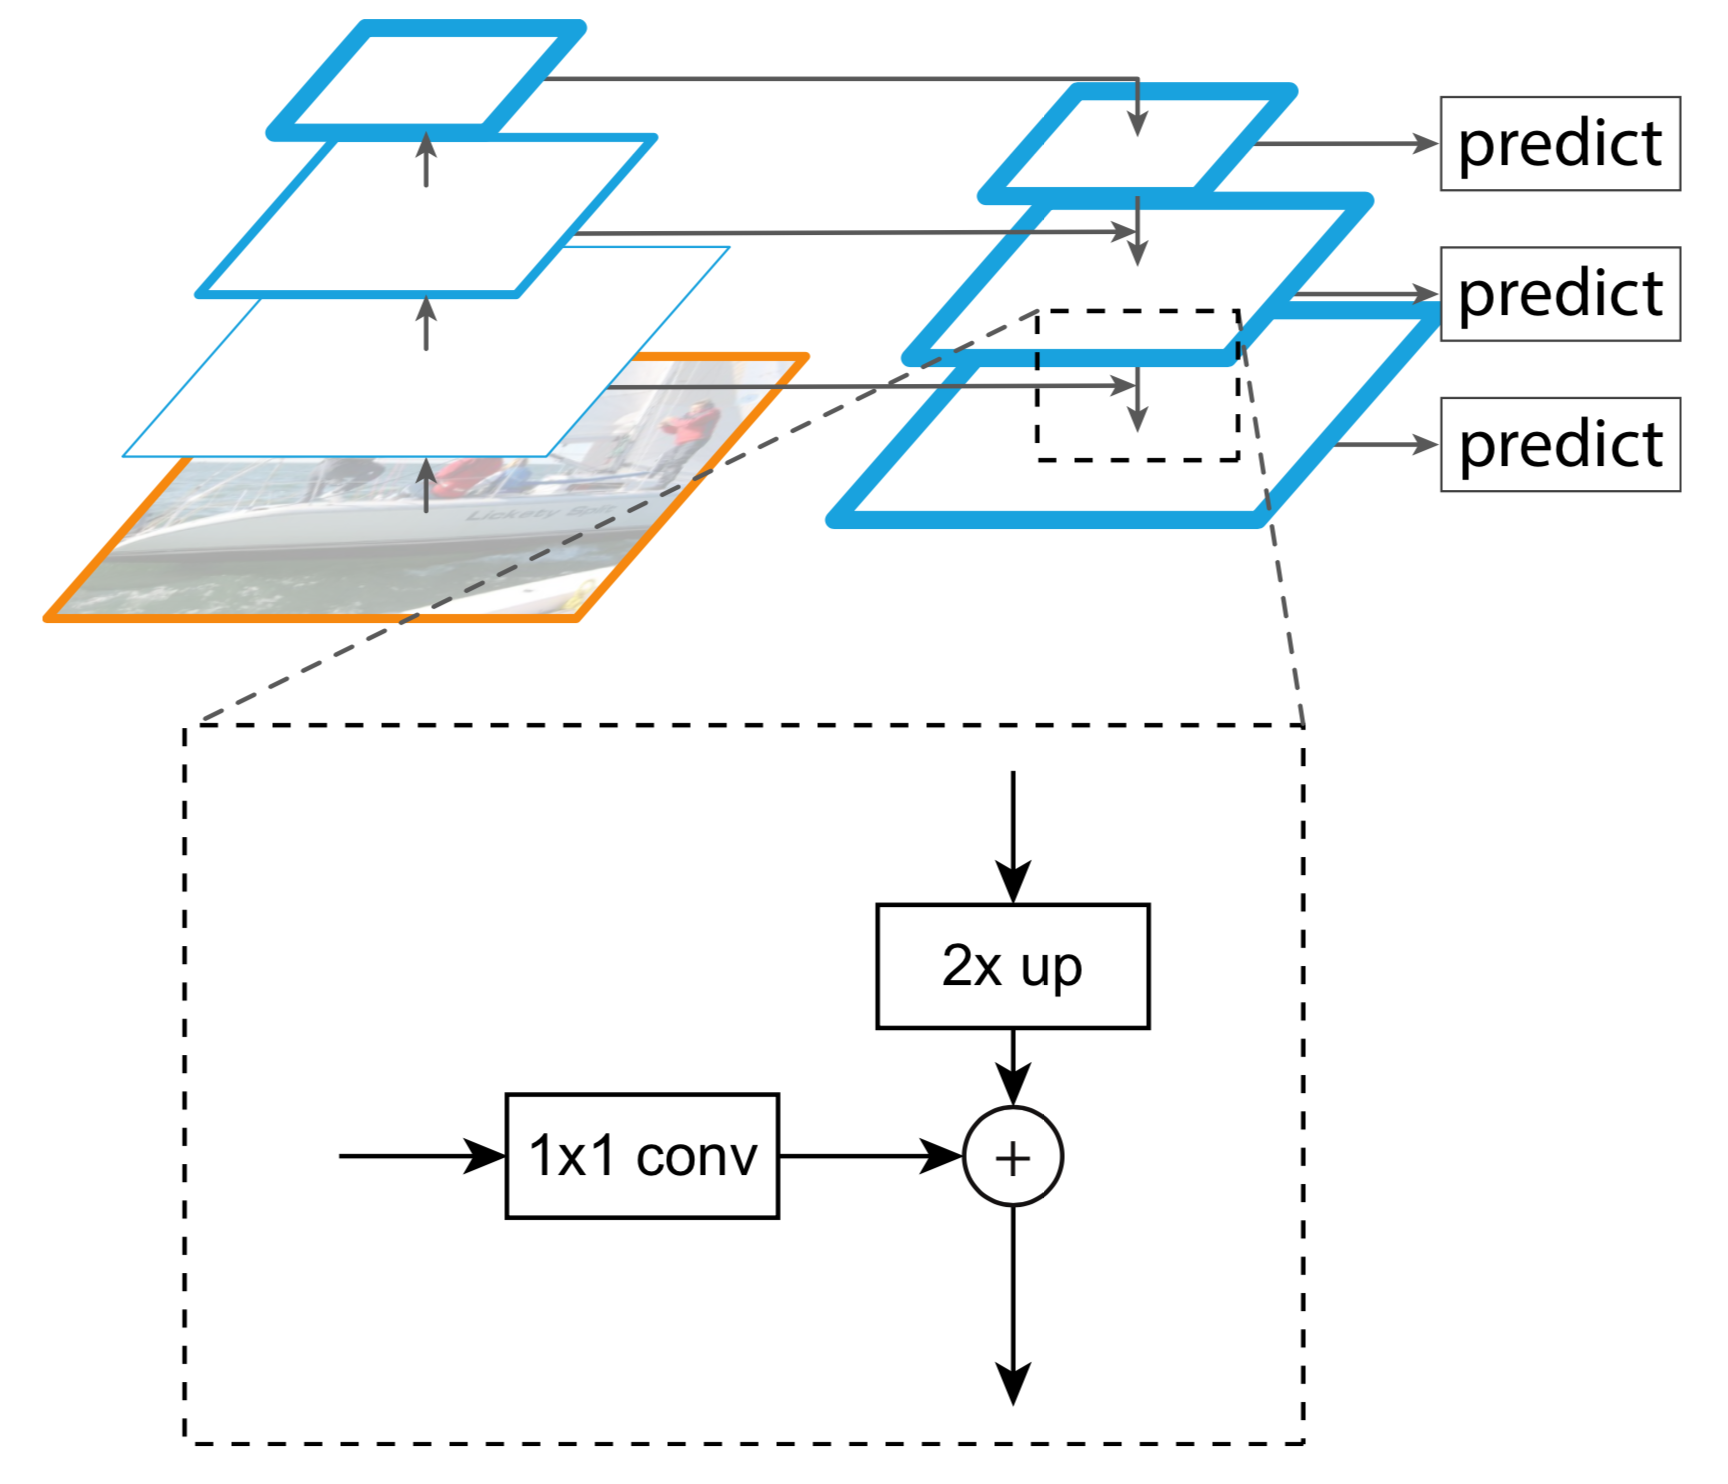
\includegraphics[width=6cm]{images/ch2/fig10.png}
  \caption{Top-down building block in RetinaNet and FPN. Reproduced from \cite{lin2017feature}}
  \label{fig10}
\end{figure} 

In fact, instead of featurising the output layers in each convolutional block, RetinaNet, attaches in the end of the backbone network two more \textbf{$3\times3$ strided convolutional layers}, continuing downscaling by the same factor the output, without making use of pooling. These outputs are noted as $C_6,C_7$ and the featurised levels are the set $(C_3, C_4, C_5, C_6, C_7)$ which produce the output pyramidal layers $(P_3, P_4, P_5, P_6, P_7)$.

\subsection{Anchor boxes}
RetinaNet, adapts the anchor boxes concept to produce RoIs in contrast with the FPN which uses a region proposal network. Due to the number of pooling operations every pyramidal level has underwent, the stride in each $P_i$ layer is $(8, 16, 32, 64, 128)$\footnote{$P_3$ has already been pooled 3 times from block$_1$, block$_2$ and block$_3$, thus it has a stride of $2^3$.}. The effective receptive field of each layer is crucial and act as a limiting factor for the size of the anchors and the size of the detected object as a consequence; stride on the other hand, indicates the density of the predictions. However, in RetinaNet this is not completely true as each $P_i$ is product of many layer outputs, from various depths with different receptive fields. In general, spatially large $P_i$ features aim in dense small object detection, while coarser $P_i$ maps are responsible for large object detection. Specifically, each layer has anchors in three scales and three ratios. Anchor's base size is $(32^2, 64^2, 128^2, 256^2, 512^2)$ with scales $(2^0, 2^{1/3}, 2^{2/3})$ and ratios of $(1\!:\!2,1\!:\!1,2\!:\!1)$.

\subsection{Prediction subnet}
The subnetwork responsible for detections consist of a \textbf{classification subnet} and a \textbf{box regression subnet}. The classification subnet predicts $p(c_i)$, out of K classes, in each anchor position and is nothing more than 4 stacked $3\times3\times C$ convolutional kernels with ReLU activations, followed by  $3\times3\times KA$ with sigmoid activation. C is the channel depth of $P_i$ and is the same all layers.

The class agnostic box regression subnet, follows the same logic with 4 stacked $3\times3\times C$ convolutional kernels with ReLU activations, followed by $3\times3\times 4A$ with sigmoid activation. The output is a four-tuple for every anchor position with the refined bounding box. The prediction subnet shares its parameters across all pyramidal $P_i$ outputs, following the same philosophy as SSD.

\section{Evaluation Metrics}
Object detection has several evaluation metrics, however performance comparisons depend on the problem. For example in the PASCAL VOC challenge, models compete between those with the highest mAP, while in the apple detection problem a model with higher F1-score is more accurate. However the most useful metrics are:

\bigskip
\textbf{Recall}
\bigskip\noindent
\begin{equation}
  \text{Recall} = \frac{TP}{TP+FN}=\frac{TP}{\text{Num. of objects}}
\end{equation} 
Recall is the fraction between successfully detected instances and the number of instances.

\bigskip
\textbf{Precision}
\bigskip\noindent
\begin{equation}
  \text{Precision} = \frac{TP}{TP+FP}=\frac{TP}{\text{Predictions}}
\end{equation} 
Precision gives the ability of the model identifying only the relevant instances as it gets lower for every wrong prediction.

\bigskip
\textbf{F1-score}
\bigskip\noindent
\begin{equation}
  \text{F1-score} = 2\times\frac{\text{Precision}\times \text{Recall}}{\text{Precision}+\text{Recall}}\end{equation} 
F1-score is the harmonic mean between precision in recall, giving equal importance in both. It is mostly used in tasks where the model should find the best ratio between true positives and false positives. Changing detector's confidence threshold comes with an expense in the rate of true positives along with the rate of false negatives. F1-score indicates the point in the precision-recall curve where precision and recall have the maximum values.

%\bigskip
%\textbf{Average Precision}
%\bigskip\noindent
%Average precision is the area under curve (AUC) of the precision - recall curve. The PR curve follows usually a zigzag pattern complicating its calculation. \cite{everingham2010pascal}, proposed an alternative way in its calculation by interpolating precision in 11 evenly space points. The precision at each recall level takes the maximum value in order to eliminate the zigzag pattern.
%\begin{equation}
%  \text{AP} = \frac{1}{11}\sum_{r\in\{0,0.1,...,1\}}p_{interp}(r) \\
%  p_{interp}(r)=\max_{\hat{r}:\hat{r}\geq r}p(\hat{r})
%\end{equation} 
\dots